\subsection{Delegable Prove}\label{section: zkzkvm-delegable-prove}

The Section \ref{section: zkzkvm-user-end-prove} scheme highlights a key challenge in generating cryptographic proofs for transactions in a blockchain network. As the complexity of the transaction and the number of calls involved increases, so does the cost of creating and including the proof in the transaction. This poses a significant problem for users, particularly those using weaker devices such as mobile phones or hardware tokens.

To address this issue, a solution called Delegable Prove Scheme (DPS) has been proposed. DPS allows users to delegate the task of generating cryptographic proofs to a third party, such as a server or a more powerful device, while still maintaining the security and validity of the transaction. This means that users can conduct complex transactions without incurring the high cost of generating proofs themselves.

The key system and note design used in DPS ensures that transactions remain private and secure, even when proof generation is delegated to a third party. The system creates notes, which represent a certain unit of state, and each note is assigned a unique key. When a user wants to send a private transaction, they create a new note with a new stealth key and send it to the receiver. To ensure that the transaction is valid, a cryptographic proof is required to show that the note has not been previously spent or duplicated.

\subsubsection{Current design}

We compared the proof generation schemes of ZCash \cite{website:zcash-nu5}, ZEXE \cite{cryptoeprint:2018/962}, VERI-ZEXE \cite{cryptoeprint:2022/802}, Aleo \cite{website:aleo-vm}, and Aztec \cite{website:aztec3}, as shown in the diagram \ref{fig:cur_proof_generation} below:
\begin{figure}[!ht]
    \centering
    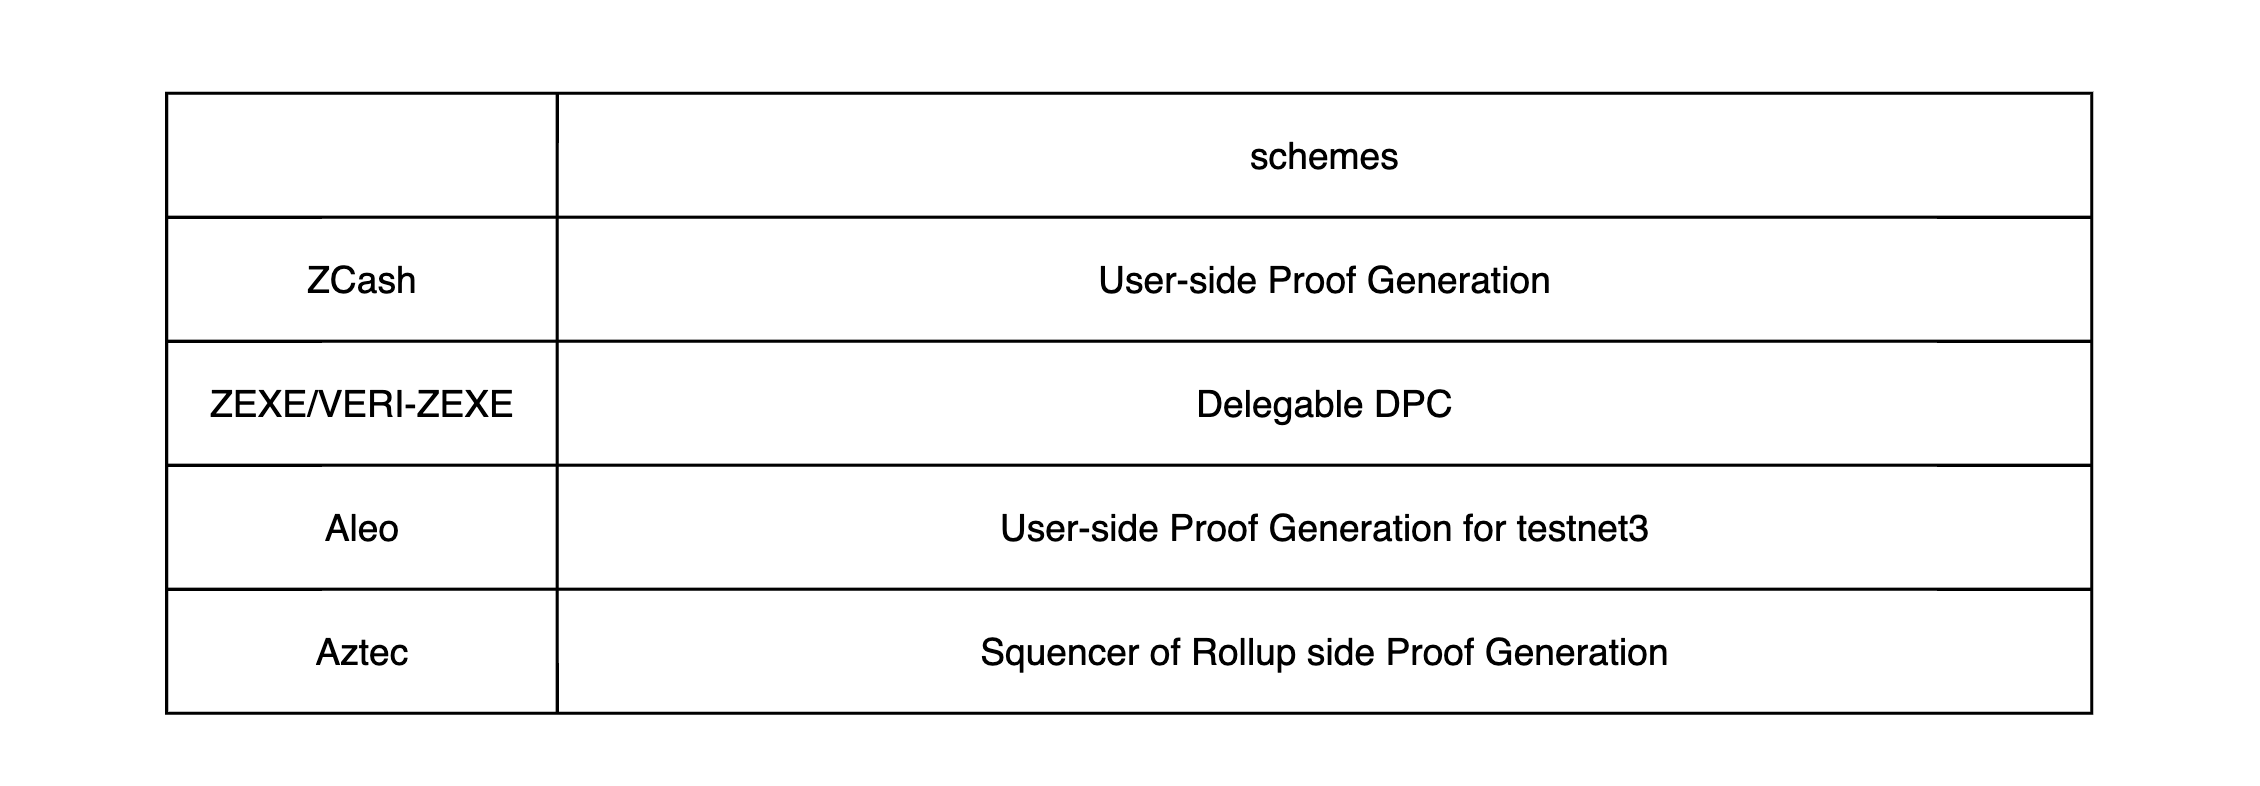
\includegraphics[width=0.8\textwidth]{cur_proof_generation.png}
    \caption{Current Proof Generation Schemes}
    \label{fig:cur_proof_generation}
\end{figure}

\subsubsection{Our work}